\documentclass{standalone}
\usepackage{tikz}
\usepackage{tikzscale}
\usetikzlibrary{arrows}
\usetikzlibrary{arrows.meta}
\usetikzlibrary{patterns}
\usetikzlibrary{shapes}
\usetikzlibrary{calc}
\usetikzlibrary{matrix}
\usetikzlibrary{positioning}
\usepackage{calc}
\usetikzlibrary{calc,trees,positioning,arrows,fit,shapes}

\usepackage{tkz-euclide}
\usetikzlibrary{
	angles,
	quotes,
}
\usepackage{pgfplots}

\begin{document}
	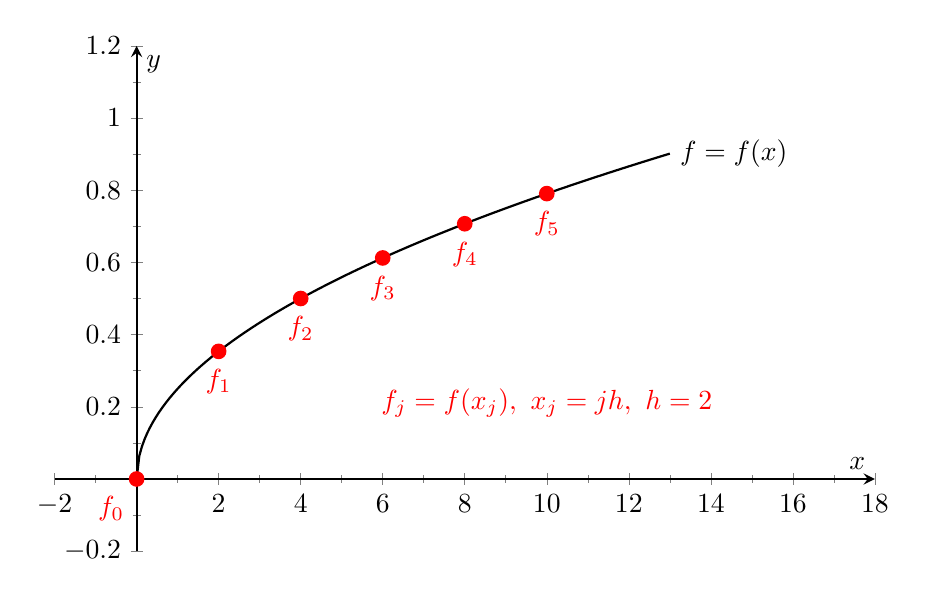
\begin{tikzpicture}%[scale=0.6]
\begin{axis}[set layers = standard,
xmin = -2, xmax = 18,
ymin = -0.2, ymax = 1.2,    
minor tick num = 1,        
axis lines=center,
axis line style = thick,          
xlabel = {$x$},
ylabel = {$y$},
disabledatascaling,
%axis equal,
width=12cm,
height=8cm	        
%width=0.9\textwidth,
%height=\textheight	        
]
\draw[domain = 0:13, thick, black, samples = 200,] plot(\x, 0.25*\x^0.5) node[right] {$f=f(x)$};
\node[label={[text=red]250:$f_0$},circle,fill,red,inner sep=2.0pt] at (axis cs:0,0.25*0^0.5) {};  
\node[label={[text=red]270:$f_1$},circle,fill,red,inner sep=2.0pt] at (axis cs:2,0.25*2^0.5) {};  
\node[label={[text=red]270:$f_2$},circle,fill,red,inner sep=2.0pt] at (axis cs:4,0.25*4^0.5) {};  
\node[label={[text=red]270:$f_3$},circle,fill,red,inner sep=2.0pt] at (axis cs:6,0.25*6^0.5) {};  
\node[label={[text=red]270:$f_4$},circle,fill,red,inner sep=2.0pt] at (axis cs:8,0.25*8^0.5) {};  
\node[label={[text=red]270:$f_5$},circle,fill,red,inner sep=2.0pt] at (axis cs:10,0.25*10^0.5) {};  

\node[label={[text=red]270:${f_j=f(x_j),~x_j=jh,~h=2}$},circle,red,inner sep=2.0pt] at (axis cs:10,0.3) {};
\end{axis}
\end{tikzpicture}
	
\end{document}